The processor architecture is a MIPS-inspired pipelined architecture with five stages.
The five stages are called Instruction Fetch, Instruction Decode, Execution, Memory and Write Back.
Each stage is separated by pipeline registers that hold the relevant data for the different stages between clock cycles.
With a pipelined design, the processor is vulnerable to data hazards and control hazards \todo{explain what hazards are somewhere?}.
The processor resolves hazards by using a combination of data forwarding and stalling.
One type of hazard, the use-after-load\cn hazard is not handled by the processor, and trying to execute an instruction which uses the result from a load immediately after the load instruction results in undefined behaviour.
Instead of handling this in hardware, the bundled solution assembler solves this issue by instruction reordering, or simply inserting nops where needed.

The processor architecture is modeled after the Harvard Architecture design, which means that it has separate instruction and data memory.
This, in addition to being a security boon, makes for a more performant design, as the instruction memory and data can be accessed independantly.
This is aligned with the performance design goal.
This removes the need for a central memory access arbitrage unit, which increases the simplicty of the design in accordance to the design goals\cn.

The processor architecture can bee seen illustrated in figure \vref{figure:architecture}.
The tall orange bars are the pipeline registers.
The blue lines are control signals.

\begin{figure}[H]
    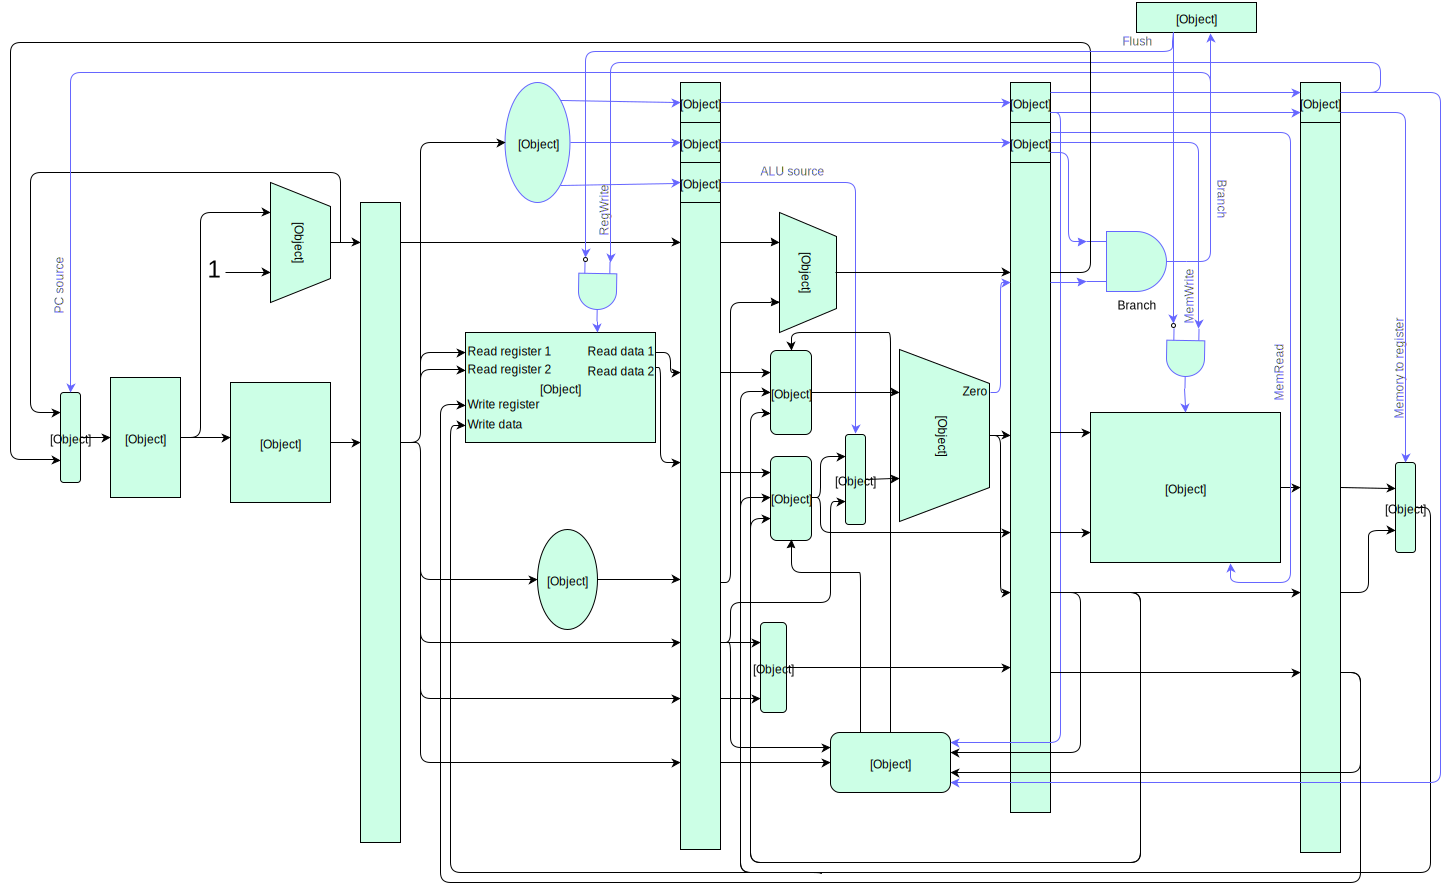
\includegraphics[width=\textwidth]{illustrations/processor.pdf}
    \caption{The processor architecture}
    \label{figure:architecture}
\end{figure}


The rest of this section describes the different architectural subcomponents in detail.

\subsection{Instruction Fetch Stage}
    \todo{image of fetch stage}

The instruction fetch stage is the first stage in the processor pipeline.
It is responsible for fetching the correct instruction from the instruction memory, and feeding it to the next stage in the pipeline.

\subsubsection{Program Counter}
In order to know where in the program the processor is currently executing, a program counter is needed.
The program counter is a simple register which holds the instruction address of the address currently being fetched and sent on to the next stage in the pipeline.
The instruction fetch stage updates the program counter each cycle, either by increasing it by one so as to fetch the next instruction, or by to a different number requested by a different part of the processor, in the case of a jump.



\subsection{Instruction Decode Stage}
    \todo{picture of decode stage}

The instruction decode stage receives an instruction from the instruction fetch stage and understands it.
Using this understanding, it orchestrates and coordinates the execution of the instruction.
This means that it is responsible for preparing the necessary data for the ALU, and setting the appropriate control signals for the rest of the processor for each instruction.
The register file of the processor resides in the instruction decode stage, and register data that are needed in computation in the execution stage are fetched and prepared in the instruction decode stage.
The control unit also resides in this stage.

\newpage
\subsubsection{Register File}
    The register file is a large block of 32 registers that make up the general purpose registers of the processor that are accessible to users.
The register file implementation is the same as in the prevous assignment\cn, and is also part of the supploed support files for this assignment\cn.


\newpage
\subsubsection{Control Unit}
    The control unit is the component that is responsible for enabling and disabling the correct parts of the processor at the correct times, so that an instruction is executed correctly.

\subsubsection{In Signals}

\begin{description}
\item{\textbf{Instruction Op-code}} \\
    The op-code of the currently executing instruction in the instruction decode stage.

\item{\textbf{Instruction Function}} \\
    The ALU function of the currently executing instruction in the instruction decode stage. 
\end{description}

\subsubsection{Out Signals}

\begin{description}
\item{\textbf{Execute Control Signals}} \\
    The control signals that should be used in the execute stage for the instruction being decoded by the control unit.
    The execute control signals bus contains the \textbf{ALU Source}, \textbf{ALU Function} and \textbf{Register Destination} control signals.

\item{\textbf{Memory Control Signals}} \\
    The control signals that should be used in the memory stage for the instruction being decoded by the control unit.
    The memory control signals bus contains the \textbf{Branch}, \textbf{Jump} and \textbf{Memory Write} control signals.

\item{\textbf{Write-Back Control Signals}} \\
    The control signals that should be used in the write-back stage for the instruction being decoded by the control unit.
The write-back control signals bus contains the \textbf{Memory to Register} and \textbf{Register Write} control signals.
\end{description}




\subsection{Execution Stage}
    The execution stage is where the magic happens.
It is responsible for executing the instructions.
The ALU is located in this stage.
The execution stage also contains some important hazard-correcting circuitry.

\subsubsection{ALU}
    The ALU, or the arithmetic logic unit, is the heart of the processor.
The ALU is responsible for doing actual arithmetic and logical operations on data.
The rest of the processor is in reality machinery working to feed the ALU with as much data as quickly as possible.
It is therefore important that the ALU can work as fast as possible, in accordance to the performance design goal from section\vref{subsection:performance}.
The processor uses dedicated DSP slices on the FPGA to speed up the performance of the ALU.

\subsubsection{In Signals}

\begin{description}
\item{\textbf{Y}} \\
The first operand of an ALU operation.

\item{\textbf{X}} \\
The second operand of an ALU operation.

\item{\textbf{Function}} \\
The function code that decides which operation the ALU should perform on $ X $ and $ Y $.
\end{description}

\subsubsection{Out Signals}

\begin{description}
\item{\textbf{Result}} \\
    The result of the ALU operation.

\item{\textbf{Zero}} \\
    A Boolean value which is set if the result of the ALU operation is 0, or unset if the result of the ALU operation is not zero.
    This signal is used for determining the outcome of comparisons, so that they may be used in conditionals.
\end{description}


\subsubsection{Forwarding Unit}
    \todo{The Forwarding Unit description}

\subsubsection{In Signals}

\begin{description}
\item{\textbf{rs\_address\_from\_id\_ex}} \\
Description of it.
\item{\textbf{rt\_address\_from\_id\_ex}} \\
Description of it.
\item{\textbf{register\_destination\_from\_ex\_mem}} \\
Description of it.
\item{\textbf{register\_destination\_from\_mem\_wb}} \\
Description of it.
\item{\textbf{register\_write\_from\_ex\_mem}} \\
Description of it.
\item{\textbf{register\_write\_from\_mem\_wb}} \\
Description of it.
\end{description}

\subsubsection{Out Signals}

\begin{description}
\item{\textbf{forward\_rs\_out}} \\
Description of it.
\item{\textbf{forward\_rt\_out}} \\
Description of it.
\end{description}


\subsubsection{Hazard Detector}
    \todo{The Hazard Detector description}

\subsubsection{In Signals}

\begin{description}
\item{\textbf{register\_address\_in}} \\
Description of it.
\item{\textbf{register\_write\_execute\_in}} \\
Description of it.
\item{\textbf{register\_write\_memory\_in}} \\
Description of it.
\item{\textbf{register\_destination\_execute\_in}} \\
Description of it.
\item{\textbf{register\_destination\_memory\_in}} \\
Description of it.
\end{description}

\subsubsection{Out Signals}

\begin{description}
\item{\textbf{hazard\_out}} \\
Description of it.
\end{description}



\subsection{Memory Stage}
    The memory stage is responsible for interfacing with the data memory in the system.
It also contains the logic which determines whether or not branches should be taken.

\subsubsection{Data Memory}

\todo{this}


\subsection{Write-Back Stage}
    The Write Back stage is responsible for routing the correct data to the register file, when data should be written to the register file.


\subsection{Additional Components}
    \subsubsection{Pipeline Registers}
\todo{this}

\subsubsection{Flip Flop}
\todo{this}

\subsubsection{Multiplexors}
\todo{this}
\subsubsubsection{Mux 2}
\subsubsubsection{Mux 3}

